\documentclass[nooutcomes]{ximera}
%\documentclass[space,handout,nooutcomes]{ximera}

% For preamble materials

\usepackage{pgf,tikz}
\usepackage{mathrsfs}
\usetikzlibrary{arrows}
\usepackage{framed}
\usepackage{amsmath}
\pgfplotsset{compat=1.17}

\def\fixnote#1{\begin{framed}{\textcolor{red}{Fix note: #1}}\end{framed}}  % Allows insertion of red notes about needed edits
%\def\fixnote#1{}

\def\detail#1{{\textcolor{blue}{Detail: #1}}}   

\pdfOnly{\renewenvironment{image}[1][]{\begin{center}}{\end{center}}}

\graphicspath{
  {./}
  {chapter1/}
  {chapter2/}
  {chapter4/}
  {proofs/}
  {graphics/}
  {../graphics/}
}

\newenvironment{sectionOutcomes}{}{}


%%% This set of code is all of our user defined commands
\newcommand{\bysame}{\mbox{\rule{3em}{.4pt}}\,}
\newcommand{\N}{\mathbb N}
\newcommand{\C}{\mathbb C}
\newcommand{\W}{\mathbb W}
\newcommand{\Z}{\mathbb Z}
\newcommand{\Q}{\mathbb Q}
\newcommand{\R}{\mathbb R}
\newcommand{\A}{\mathbb A}
\newcommand{\D}{\mathcal D}
\newcommand{\F}{\mathcal F}
\newcommand{\ph}{\varphi}
\newcommand{\ep}{\varepsilon}
\newcommand{\aph}{\alpha}
\newcommand{\QM}{\begin{center}{\huge\textbf{?}}\end{center}}

\renewcommand{\le}{\leqslant}
\renewcommand{\ge}{\geqslant}
\renewcommand{\a}{\wedge}
\renewcommand{\v}{\vee}
\renewcommand{\l}{\ell}
\newcommand{\mat}{\mathsf}
\renewcommand{\vec}{\mathbf}
\renewcommand{\subset}{\subseteq}
\renewcommand{\supset}{\supseteq}
%\renewcommand{\emptyset}{\varnothing}
%\newcommand{\xto}{\xrightarrow}
%\renewcommand{\qedsymbol}{$\blacksquare$}
%\newcommand{\bibname}{References and Further Reading}
%\renewcommand{\bar}{\protect\overline}
%\renewcommand{\hat}{\protect\widehat}
%\renewcommand{\tilde}{\widetilde}
%\newcommand{\tri}{\triangle}
%\newcommand{\minipad}{\vspace{1ex}}
%\newcommand{\leftexp}[2]{{\vphantom{#2}}^{#1}{#2}}

%% More user defined commands
\renewcommand{\epsilon}{\varepsilon}
\renewcommand{\theta}{\vartheta} %% only for kmath
\renewcommand{\l}{\ell}
\renewcommand{\d}{\, d}
\newcommand{\ddx}{\frac{d}{dx}}
\newcommand{\dydx}{\frac{dy}{dx}}


\usepackage{bigstrut}


\title{Quadrilaterals}
\author{Brad Findell}
\begin{document}
\begin{abstract}
A few proofs about quadrilaterals. 
\end{abstract}
\maketitle


\begin{problem}
Adapted from Ohio's 2017 Geometry released item 13. 

Two pairs of parallel lines intersect to form a parallelogram as shown.  
\begin{image}
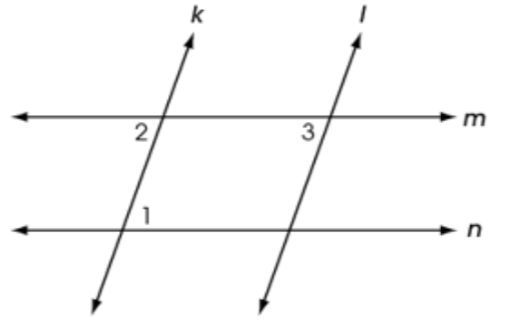
\includegraphics{Q13.png}
\end{image}
Complete the following proof that opposite angles of a parallelogram are congruent: 

\begin{enumerate}
\item $\angle 1 \cong \angle 2$ as \wordChoice{\choice{opposite angles}\choice[correct]{alternate interior angles}\choice{corresponding angles}}
for parallel lines \wordChoice{\choice[correct]{$m$ and $n$}\choice{$k$ and $l$}}.
\item $\angle 3 \cong \angle 2$ as \wordChoice{\choice{opposite angles}\choice{alternate interior angles}\choice[correct]{corresponding angles}}for parallel lines \wordChoice{\choice{$m$ and $n$}\choice[correct]{$k$ and $l$}}.
\item Then $\angle 1 \cong \angle 3$ because they are both congruent 
to $\angle 2$. 
\end{enumerate}
\end{problem}

\begin{problem}
Adapted from Ohio's 2018 Geometry released item 21. 

Given the parallelogram $WXYZ$, prove that $\overline{WX}\cong\overline{YZ}$. 

\begin{image}
\definecolor{qqqqff}{rgb}{0.,0.,1.}
\begin{tikzpicture}[line width=0.8pt,line cap=round,line join=round,x=1.0cm,y=1.0cm] % ,>=triangle 45
\clip(-0.5,-0.6) rectangle (5.5,2.5);
\draw (0.,0.)-- (4.,0.);
\draw (4.,0.)-- (5.,2.);
\draw (5.,2.)-- (1.,2.);
\draw (1.,2.)-- (0.,0.);
\draw (1.,2.)-- (4.,0.);
\begin{scriptsize}
\draw [fill=qqqqff] (0.,0.) circle (1.2pt);
\draw[color=qqqqff] (-0.28,-0.03) node {$Z$};
\draw [fill=qqqqff] (1.,2.) circle (1.2pt);
\draw[color=qqqqff] (0.86,2.29) node {$W$};
\draw[color=qqqqff] (1.08,1.75) node {$1$};
\draw[color=qqqqff] (1.5,1.87) node {$2$};
\draw [fill=qqqqff] (4.,0.) circle (1.2pt);
\draw[color=qqqqff] (4.24,-0.03) node {$Y$};
\draw[color=qqqqff] (3.5,0.15) node {$3$};
\draw[color=qqqqff] (3.9,0.3) node {$4$};
\draw [fill=qqqqff] (5.,2.) circle (1.2pt);
\draw[color=qqqqff] (5.14,2.29) node {$X$};
\draw[color=white] (-3,0) circle (0.2pt);
\draw[color=white] (8,0) circle (0.2pt);
\end{scriptsize}
\end{tikzpicture}
\end{image}


Complete the proof below: 
\begin{enumerate}
\item $\angle 1 \cong \angle 4$ as \wordChoice{\choice[correct]{alternate interior angles}\choice{corresponding angles}\choice{opposite angles}} for parallel segments \wordChoice{\choice[correct]{$\overline{WZ}$ and $\overline{XY}$}\choice{$\overline{WX}$ and $\overline{YZ}$}}.
\item $\angle 2 \cong \angle 3$ for the same reason, this time for parallel segments \wordChoice{\choice{$\overline{WZ}$ and $\overline{XY}$}\choice[correct]{$\overline{WX}$ and $\overline{YZ}$}}.
\item $\overline{WY}\cong\overline{YW}$ because a segment is congruent to itself. 
\item $\triangle WYZ \cong \triangle \answer[format=string]{YWX}$ by \wordChoice{\choice{SAS}\choice[correct]{ASA}\choice{SSS}}.  
\item Then $\overline{YZ}\cong\overline{WX}$ as corresponding parts of congruent triangles. 
\end{enumerate}

\end{problem}

\newpage
\begin{problem}
Kites can often be found behind basic constructions because of important 
\wordChoice{\choice{definitions}\choice{measurements}\choice[correct]{properties}}
of their \wordChoice{\choice{sides}\choice[correct]{diagonals}\choice{angles}}.  

Quadrilateral $ABCD$ is a kite as marked.  Prove that $\overleftrightarrow{BD}$ is the perpendicular bisector of $\overline{AC}$. 
\begin{image}
\definecolor{qqqqff}{rgb}{0.,0.,1.}
\begin{tikzpicture}[scale= 0.8, line cap=round,line width=0.8pt,line join=round,>=triangle 45,x=1.0cm,y=1.0cm]
\clip(-5,-5.3) rectangle (5,2.5);
\draw (-3.,0.)-- (0.,-5.);
\draw (-1.440,-2.424) -- (-1.595,-2.516);
\draw (-1.405,-2.484) -- (-1.559,-2.576);
\draw (0.,-5.)-- (3.,0.);
\draw (1.405,-2.484) -- (1.559,-2.576);
\draw (1.440,-2.424) -- (1.595,-2.516);
\draw (3.,0.)-- (0.,2.);
\draw (1.450,0.925) -- (1.550,1.075);
\draw (0.,2.)-- (-3.,0.);
\draw (-1.450,0.925) -- (-1.550,1.075);
\draw (0.,2.)-- (0.,-5.);
\draw (-3.,0.)-- (3.,0.);
\draw (0.,2.)-- (3.,0.);
%\begin{scriptsize}
\draw [fill=qqqqff] (-3.,0.) circle (1.2pt);
\draw[color=qqqqff] (-3.24,0.31) node {$A$};
\draw [fill=qqqqff] (3.,0.) circle (1.2pt);
\draw[color=qqqqff] (3.22,0.21) node {$C$};
\draw [fill=qqqqff] (0.,2.) circle (1.2pt);
\draw[color=qqqqff] (0.14,2.29) node {$B$};
\draw [fill=qqqqff] (0.,-5.) circle (1.2pt);
\draw[color=qqqqff] (-0.26,-5.09) node {$D$};
%\draw [fill=qqqqff] (0.,0) circle (1.2pt);
%\draw[color=qqqqff] (-0.26,-.26) node {$X$};
\draw[color=qqqqff] (-5,0) circle (0.2pt);
\draw[color=qqqqff] (8,0) circle (0.2pt);
%\end{scriptsize}
\end{tikzpicture}
\end{image}

\begin{hint}
Theorem:  The points on a perpendicular bisector are exactly those that are equidistant from the endpoints of a segment.  
\end{hint}

Proof:  Because $B$ is $\answer[format=string]{equidistant}$ from $A$ and $C$, it must lie on the perpendicular bisector of segment $\answer{AC}$.  And because $D$ is
 $\answer[format=string]{equidistant}$ from $A$ and $C$, it also must lie on the perpendicular bisector of segment $\answer{AC}$.  
 Because two (distinct) points determine a line, $\overleftrightarrow{BD}$ must be the (unique) perpendicular bisector of $\answer{AC}$.  

\begin{problem}
Correct!  It helps to think of a kite can as formed by two $\answer[format=string]{isosceles}$ triangles with a common base. 
\end{problem}
\end{problem}

\newpage 

\begin{problem}
Quadrilateral $ABCD$ is a kite as marked.  Prove that $\overleftrightarrow{BD}$ is the perpendicular bisector of $\overline{AC}$. 

\begin{image}
\definecolor{qqqqff}{rgb}{0.,0.,1.}
\begin{tikzpicture}[scale = 0.8, line cap=round,line width=0.8pt,line join=round,>=triangle 45,x=1.0cm,y=1.0cm]
\clip(-5,-5.3) rectangle (5,2.5);
\draw (-3.,0.)-- (0.,-5.);
\draw (-1.440,-2.424) -- (-1.595,-2.516);
\draw (-1.405,-2.484) -- (-1.559,-2.576);
\draw (0.,-5.)-- (3.,0.);
\draw (1.405,-2.484) -- (1.559,-2.576);
\draw (1.440,-2.424) -- (1.595,-2.516);
\draw (3.,0.)-- (0.,2.);
\draw (1.450,0.925) -- (1.550,1.075);
\draw (0.,2.)-- (-3.,0.);
\draw (-1.450,0.925) -- (-1.550,1.075);
\draw (0.,2.)-- (0.,-5.);
\draw (-3.,0.)-- (3.,0.);
\draw (0.,2.)-- (3.,0.);
%\begin{scriptsize}
\draw [fill=qqqqff] (-3.,0.) circle (1.2pt);
\draw[color=qqqqff] (-3.24,0.31) node {$A$};
\draw [fill=qqqqff] (3.,0.) circle (1.2pt);
\draw[color=qqqqff] (3.22,0.21) node {$C$};
\draw [fill=qqqqff] (0.,2.) circle (1.2pt);
\draw[color=qqqqff] (0.14,2.29) node {$B$};
\draw [fill=qqqqff] (0.,-5.) circle (1.2pt);
\draw[color=qqqqff] (-0.26,-5.09) node {$D$};
\draw [fill=qqqqff] (0.,0) circle (1.2pt);
\draw[color=qqqqff] (-0.26,-.26) node {$X$};
\draw[color=qqqqff] (-5,0) circle (0.2pt);
\draw[color=qqqqff] (8,0) circle (0.2pt);
%\end{scriptsize}
\end{tikzpicture}
\end{image}

A flow-chart proof that makes use of triangle congruence:
\begin{image}
\tikzstyle{block} = [rectangle, draw, fill=blue!20, 
    text width=8em, text centered, rounded corners, minimum height=2em]
\tikzstyle{Block} = [rectangle, draw, fill=green!20, 
    text width=10em, text centered, rounded corners, minimum height=3em]
\tikzstyle{reason} = [color=gray, text width = 8 em, font = {\footnotesize}, node distance = 0.5 cm, align=right, minimum height = 1em]
\tikzstyle{implies} = [draw, -latex']
\begin{tikzpicture}[scale=0.85, transform shape, node distance = 1.5cm, auto]
    % Place nodes
    \node [Block] (a) {$\triangle BAD \cong \triangle BCD$};
    \node [reason, below of=a, node distance=0.66cm] {???};
    \node [block, left of=a, node distance = 4cm] (init) {$AD=CD$};
    \node [reason, below of=init] {Given};
    \node [block, right of=a, node distance = 4cm] (init2) {$BD=BD$};
    \node [reason, below of=init2] {Equality};
    \node [block, below of=init2] (init3) {$AB=CB$};
    \node [reason, below of=init3] {Given};
    \node [block, below of=a] (b) {$\angle ABD \cong \angle CBD$};
    \node [reason, below of=b] {CPCTC};
    \node [block, left of=b, node distance = 4cm]  (c) {$BX=BX$};
    \node [reason, below of=c] {Equality};
    \node [Block, below of=b] (d) {$\triangle ABX \cong \triangle CBX$};
    \node [reason, below of=d, node distance=0.66cm] {???};
    \node [block, below of=d] (e) {$AX=CX$};
    \node [reason, below of=e] {CPCTC};
    \node [block, below of=e] (f) {$X$ is midpoint of $\overline{AC}$};
    \node [reason, below of=f, node distance=0.66cm] {Def.};
    \node [block, right of=e, node distance = 4cm] (g) {$\angle BXA \cong \angle BXC$};    
    \node [reason, below of=g] {CPCTC};
    \node [block, right of=g, text width=10em, node distance = 4cm] (h) {$\angle BXA$ and $\angle BXC$ form a linear pair};
    \node [reason, below of=h, node distance=0.66cm] {Given};
    \node [reason, below of=b] {CPCTC};
    \node [block, below of=g] (i) {$\overline{AC}\perp\overline{BX}$ (and thus $\overleftrightarrow{BD}$)};
    \node [reason, below of=i, node distance=0.66cm] {Def.};
    \node [Block, text width=12em, below of=f] (m) 
       {Summary: $\overleftrightarrow{BD}$ is the $\perp$ bisector of $\overline{AC}$.};    
    \node [reason, below of=m, node distance=0.66cm] {Def.};
      % Draw edges
    \path [implies] (init) -- (a);
    \path [implies] (init2) -- (a);
    \path [implies] (init3) -- (a);
    \path [implies] (init3) -- (d);
    \path [implies] (a) -- (b);
    \path [implies] (b) -- (d);
    \path [implies] (c) -- (d);
    \path [implies] (d) -- (e);
    \path [implies] (e) -- (f);
    \path [implies] (d) -- (g);
    \path [implies] (g) -- (i);
    \path [implies] (h) -- (i);
    \path [implies] (f) -- (m);
    \path [implies] (i) -- (m);
\end{tikzpicture}
\end{image}
In the proof above, $\triangle BAD \cong \triangle BCD$ by $\answer[format=string]{SSS}$, and $\triangle ABX \cong \triangle CBX$ by $\answer[format=string]{SAS}$, and CPCTC means ``$\answer[format=string]{corresponding}$ parts of congruent triangles are $\answer[format=string]{congruent}$.''

\begin{problem}
For comparison, here is the same proof in a more common format:
\begin{enumerate}
\item $AB\cong CB$ and $AD\cong CD$ are given.  
\item $\overline{BD}\cong \overline{BD}$, so $\triangle BAD \cong \triangle BCD$ by SSS.  
\item $\angle ABD \cong \angle CBD$ by CPCTC. 
\item $\overline{BX}\cong \overline{BX}$, so that $\triangle ABX \cong \triangle CBX$ by SAS.  
\item $\angle BXA \cong \angle BXC$ by CPCTC, and they are a linear pair, 
so $\overline{AC}\perp\overline{BX}$ (and thus $\overleftrightarrow{BD}$ as well). 
\item $\overline{AX}\cong \overline{CX}$ by CPCTC, so $X$ is the midpoint of $\overline{AC}$.
\item Thus, $\overleftrightarrow{BD}$ is the perpendicular bisector of $\overline{AC}$.
\end{enumerate}

Observe also that from congruent triangles along the way, we can conclude that 
$\angle ABD\cong \angle \answer[format=string]{CBD}$ and $\angle ADB \cong \angle \answer[format=string]{CDB}$, 
which proves that the major diagonal $\overline{BD}$ $\answer[format=string]{bisects}$ the angles at those vertices---yet 
another reason that kites can be seen behind our basic constructions.  

\end{problem}

\end{problem}

\begin{problem}
You just completed two proofs that a diagonal of a kite is the perpendicular bisector of the other diagonal.  The first proof was about equidistant points; the second involved congruent triangles.  

Do the proofs apply to a rhombus? What about a square?  (Select all correct answers.)
\begin{selectAll}
\choice{The first proof applies to a rhombus but not a square.}
\choice{The first proof applies to a square but not a rhombus.}
\choice[correct]{The first proof applies to both a rhombus and a square.}
\choice{The first proof would require some modification for either one.}
\choice{The second proof applies to a rhombus but not a square.}
\choice{The second proof applies to a square but not a rhombus.}
\choice[correct]{The second proof applies to a both rhombus and a square.}
\choice{The second proof would require some modification for either one.}
\choice{Both proofs need to be completely rewritten.}
\end{selectAll}
\begin{problem}
Correct!  These are good reasons to prefer $\answer[format=string]{inclusive}$ definitions, so that a $\answer[format=string]{rhombus}$ is a special case of a kite and a 
$\answer[format=string]{square}$ is a special case of a rhombus.  

Even better: This theorem about kites applies to \emph{both} diagonals of a rhombus, so that we can conclude that the diagonals of a rhombus 
$\answer[format=string]{bisect}$ \emph{each other}!  

\end{problem}
\end{problem}




\end{document}
